\documentclass[11pt]{article}
%\usepackage[utf8]{inptenc}
\usepackage[letterpaper]{geometry}
\usepackage{float}
\usepackage{graphicx}
\graphicspath{{./images/}}

\begin{document}

Morgan Rosenkranz 
EECE5644 
5/2/21 

\section*{Question 1:}

To specify the minimum expected risk I used the Gaussian distributions of the two classes.
Since class 1 uses a mixture of Guassians, the denominator is a linear combination of the two: 
 
 \[
\frac{g(x\vert m_1, C_1)}{w_0 g(x\vert m_01, C_01) + w_1 g(x\vert m_02, C_02)} >< \gamma
 \]

Where the m's and C's are the corresponding means and covariences of the gaussian pdfs.
Because the distributions are equally weighted, $$w_0 = w_1 = 0.5$$.

Below I've plotted the ROC curve when using this equation and a varried $$\gamma$$ over all values of the inequality with x.
\begin{figure}[H]
	\centering
	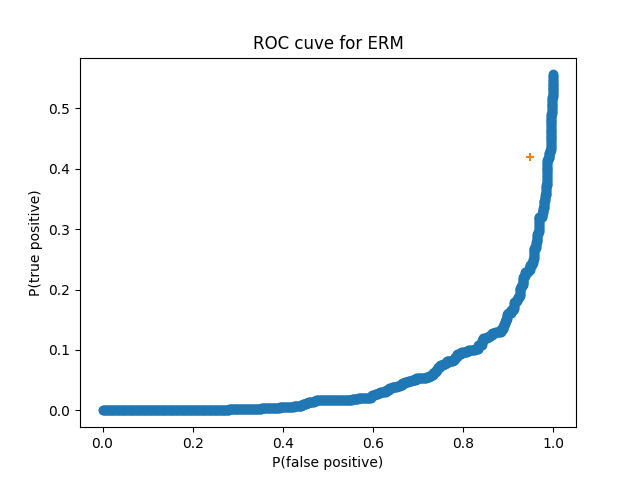
\includegraphics[width=0.75\textwidth]{ermroc}
	\caption{caption}
\end{figure}
The orange cross is the evaulation of the confusion matrix using a 0 1 loss.
The gamma value here is: asdf.
In comparison, the threshold when minimizing P(error) was 0 which would then classify all of the data into one group.

Using LDA resulted in the following P(error) and ROC curves:
\begin{figure}[H]
	\centering
	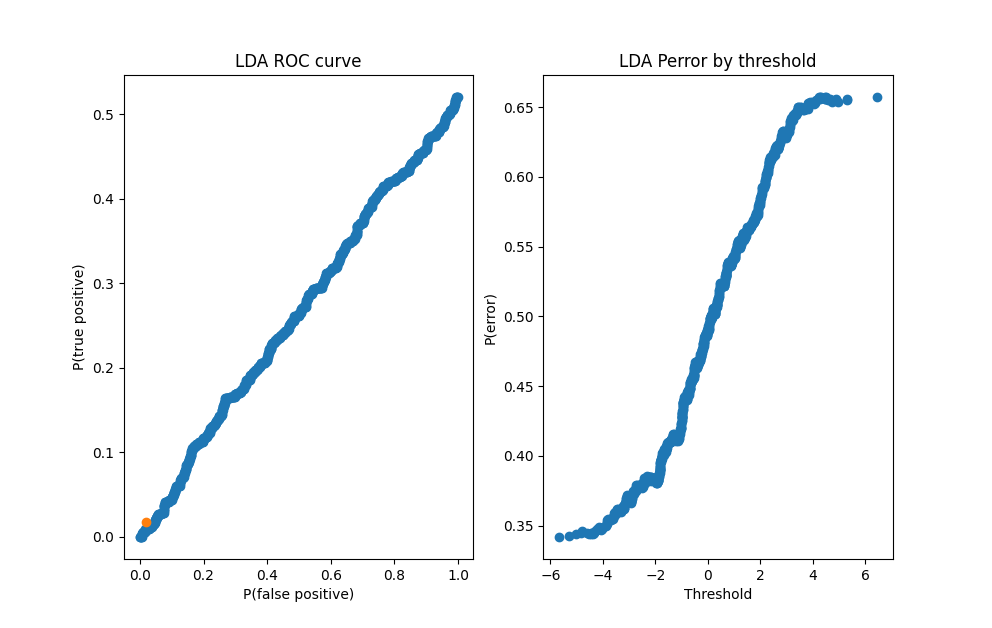
\includegraphics[width=\textwidth]{ldaroc}
	\caption{caption}
\end{figure}

The minimum perror was with a threshold of -6 whereas the threshold on the ROC curve was -4.

\section*{Question 2:}
Using the true guassian distrubutions I created 10000 samples and plotted them below.
The first two classes have their own distributions while the third comes from a mixture of two.
\begin{figure}[H]
	\centering
	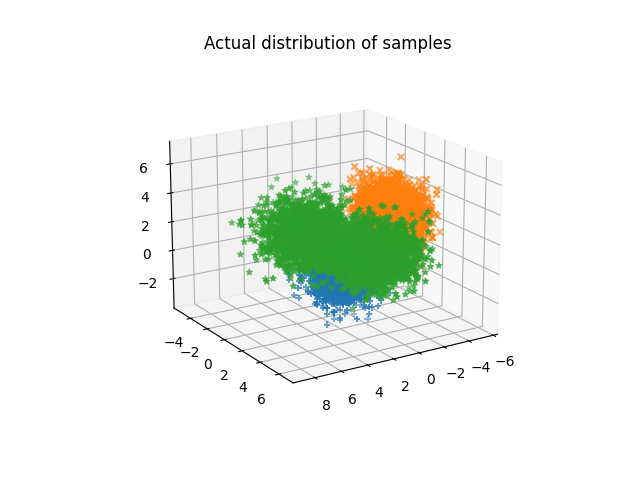
\includegraphics[width=\textwidth]{3gactual}
	\caption{Actual Distribution of Samples}
\end{figure}

Class 0 are pluses, class 1 are Xs and class 2 are all stars.

I first applied a MAP loss matrix which resulted in the following classification and confusion matrix:

\begin{figure}[H]
	\centering
	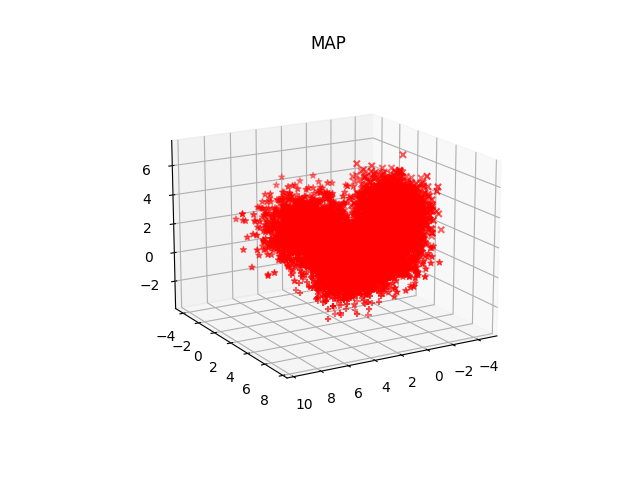
\includegraphics[width=\textwidth]{3gmap}
	\caption{MAP}
\end{figure}

0.00442177  0.99557823  0\\
0.99572509  0.00427491  0\\
0.24010948  0.75989052  0\\

One can see that using this matrix classified many elements from all classes incorrectly.

Next I used the loss matrix which cares 10 times more about being wrong:

\begin{figure}[H]
	\centering
	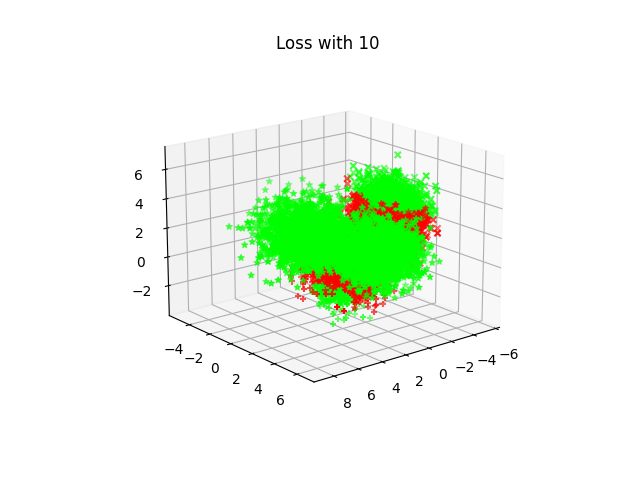
\includegraphics[width=\textwidth]{3gloss10}
	\caption{Results with Loss Matrix with Bias of 10}
\end{figure}
0.19115646 0.         0.80884354\\
0.         0.63959224 0.36040776\\
0.00223936 0.00522518 0.99253546\\

Lastly I repeated with 100:
\begin{figure}[H]
	\centering
	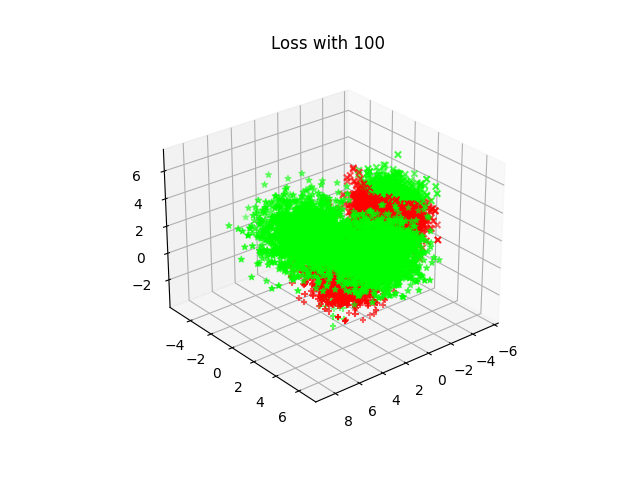
\includegraphics[width=\textwidth]{3gloss100}
	\caption{Results with Loss Matrix with Bias of 100}
\end{figure}
0.00646259 0.         0.99353741\\
0.         0.26076948 0.73923052\\
0.         0.         1.        \\

From the confusion matricies we can see that suprisingly the penalty of 10 for incorrect placement performed better on the 
first two classes than with a penalty of 100.
This may be due to the uneven distributions of the classes, where we might want to worry more about miscategorizing items
in the biggest group more than the others.

\end{document}
